\documentclass[../BTOF_summary.tex]{subfiles}
\usepackage{graphicx}
\graphicspath{Pictures}
\begin{document}


\section{Calibration}

\subsection{Ongoing Performance Monitoring}

To ensure hardware component issues are detected early the system is supposed to be monitored by small LED's mounted in between the \sipms .
Short bursts of light injected into one side of the scintillator at a time will provide a stable signal source.
Changes in the measured amplitude indicates either an efficiency loss in the scintillator or a gain drop of the involved \sipms .
These signals also act as a reference point in order to determine the time resolution of the detector elements while they are deployed.

It is foreseen to have four channels for all the LED's on one \railboard .
This allows for every other LED on a single side along the board to be illuminated, leaving a dark scintillator between two illuminated scintillators.
This ensures the signal is only produced by the internal light with no light bleed from a neighboring tile.
By only illuminating one side \todo{what is the benefit of this?}

This method needs to be improved as tests have shown that the signals measured from both sides of the scintillator tile vary in intensity, although it was assumed that these LEDs would be used for accurate measurements.
Figure 1 shows a time delay measurement.
\\
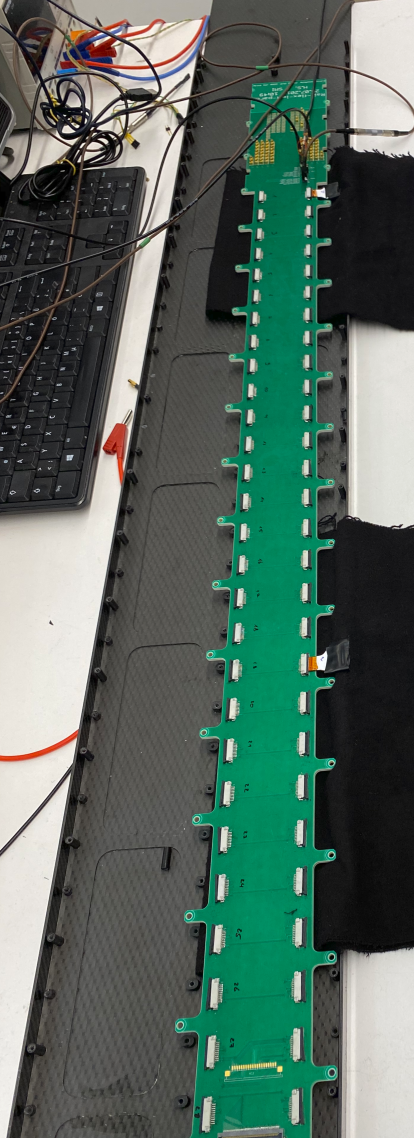
\includegraphics[scale=0.2, angle =270]{Pictures/pic1.png}
\\
\textbf{Figure 1: Tests with two LEDs on the board 1: signals measured at odd connectors 1 and 19 on the left side.}
\\

\subsection{Position Calibration}

In order to deliver useful position information for the detector hits the exact position of each tile in the context of the detector needs to be determined.\unsure{this is probably done by in the commissioning phase of the detector setup for the whole experiment.}
The position of the individual scintillator tiles is mainly of interest in the context of the time resolution, signal delay and amplitude drop along the board which are discussed in the following sections.

\subsubsection{Time Resolution Expectancy along the Board}

Since the time resolution is affected by signal noise and decreases of the slope of the rising flank it can be expected to receive a worse time resolution for scintillators farther down the \railboard\ with a longer distance between the detector element and the Front End Electronics.
In order to create a baseline for the detector performance the time resolution needs to be measured along the length of the \railboard .

\subsubsection{Signal Delay along the Board}

In order to provide an accurate time stamp for hits in the \btofD\ the time a signal needs to travel from the \sipms\ to the FEE has to be taken into account. The longer the electrical connection line is the larger the time delay between detector hit and time stamp in the electronics.

The speed a signal travels through a copper connection is significantly slower than the speed of light.

\subsubsection{Amplitude Drop along the Board}


\end{document}
